\input{../../Latex/suhw.tex}
\usepackage{graphicx,amssymb,amsmath,enumerate}
\usepackage{courier}
\usepackage{color}
\usepackage{listings}
\usepackage{fancyvrb}
\usepackage{stmaryrd}

\definecolor{dkgreen}{rgb}{0,0.6,0}
\definecolor{gray}{rgb}{0.5,0.5,0.5}
\lstset{language=Python,
	frame=lines,
   basicstyle=\ttfamily\fontsize{8}{12}\selectfont,
   keywordstyle=\color{blue},
   commentstyle=\color{red},
   stringstyle=\color{dkgreen},
   numbers=left,
   numberstyle=\tiny\color{gray},
   stepnumber=1,
   numbersep=10pt,
   backgroundcolor=\color{white},
   tabsize=2,
   showspaces=false,
   showstringspaces=false,
   lineskip=-3.5pt }
\oddsidemargin 0in
\evensidemargin 0in
\textwidth 6.5in
\topmargin -0.5in
\textheight 9.0in

\begin{document}

\project{CS255: Introduction to Cryptography}{Winter 2013}{1}{Botao Hu (botaohu@stanford.edu), Borui Wang (borui@stanford.edu)}{\today}{Encrypted Facebook groups}

\pagestyle{myheadings}  % Leave this command alone


\section{Milestone 1}

Note: In the code of this milestone, we also added MAC tags to the group messages, but we have not implemented HMAC and other mac functions yet. We'll write about MAC related issues in milestone 2. 

\subsection{How are database keys created and stored?}

When the user firsts visit facebook.com and logs in, we ask her to setup a database password. We used the database key plain text provided by the user together with a randomly generated 128 bit salt to generate a encrypted database key using PBKDF2, shown in figure \ref{fig:dbkeys}. The purpose of salt here is to add entropy to the password chosen by the user and prevent attacker to precompute rainbow tables to lookup encrypted keys. 

The encrypted database key is then used to encrypt and decrypt the group keys in the database, and is only stored in the user's sessionStorage, which means that the encrypted database key is never written to a persistent data store. The attacker will not know any information directly about the database key from the local storage. We stored the salt on the user's localStorage on disk to recalculate the encrypted database key later. If the salt is missing, we ask the user to re-setup their database. 

\begin{figure}[h!]
\centering
\caption{Setup the database password. The salt, MAC key, and MAC Tag is stored in localStorage.}
\label{fig:dbkeys}
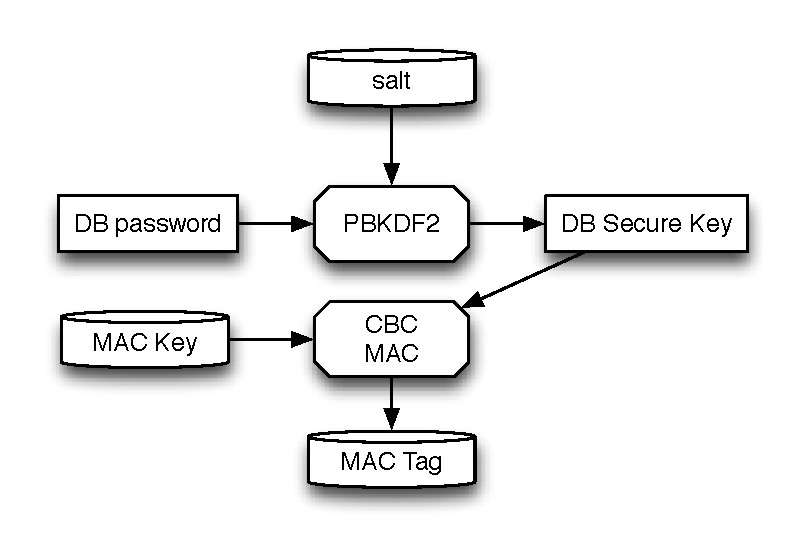
\includegraphics[height=5cm]{fig/dbkeys.eps}
\end{figure}

\subsection{How to verify if the user enters the right password?}
\label{sec:verify}
To verify if the user enters their password correctly, we generate a MAC tag (using PBKDF2) for the encrypted database key and store it in the localStorage on disk, which is illustrated in figure \ref{fig:verify_dbkeys}. Later we re-evaluate the MAC tag when user enters her password and verify if it equals to the MAC tag on localStorage. We used a randomly generated MAC key to generate the tag, where the MAC key is also stored on localStorage. Note that using MAC here is only for verification purpose and it does not prevent forgery (the attacker can use the MAC key to generate a new tag, then overwrite the tag on localStorage, but the attacker wouldn't decrypt the database correctly unless he know the database key. It can not be used to access other user's database key. Furthermore, even though the attacker may use the MAC key to find the collision of the password having the same MAC tag, but because MAC key and the salt for the database key generation are different, the attacker could not use the collision password (but different to the database password) to decrypt the database correctly. 
\begin{figure}[h!]
\centering
\caption{Verify the database password}
\label{fig:verify_dbkeys}
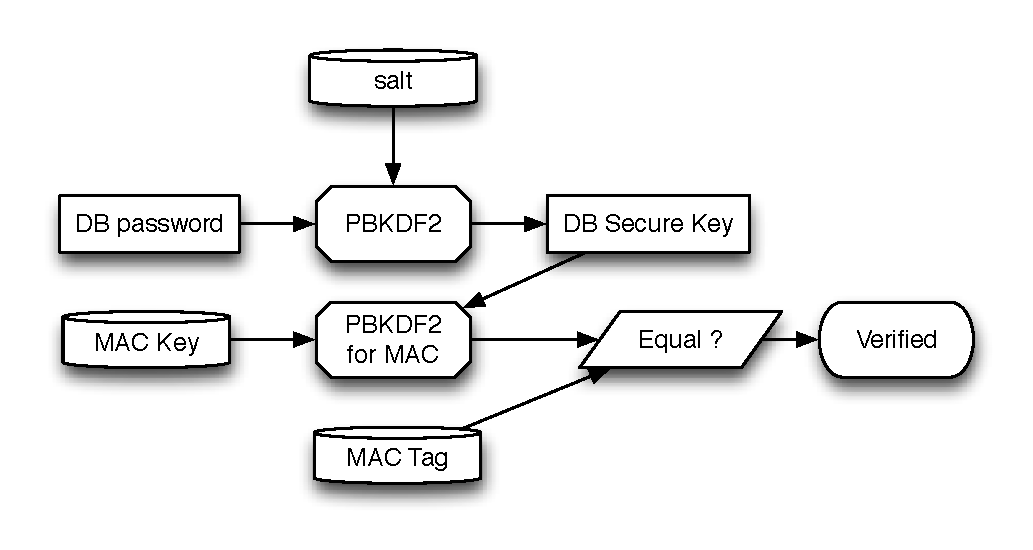
\includegraphics[height=5cm]{fig/verify_dbkeys.eps}
\end{figure}

\subsection{How to maintain a secure database for the group keys?}
We used the encrypted database keys to encrypt and decrypt groups keys on the fly without storing the encrypted database key in localStorage, which is shown in figure \ref{fig:db}. We encrypt and decrypt the group keys in nonce-based counter mode with AES.  In this way the attacker has no way to find out what the encrypted database key is given the cipher text if the block cipher under counter mode is secure. 
In addition, to prevent to leak the group name information, we encrypt and decrypt the whole JSON string of the hash table of all group keys. For integrity, we use the same MAC technology in section \ref{sec:verify} with a seperate key to ensure the integrity of the data.
\begin{figure}[h!]
\centering
\caption{Maintain the database of group keys}
\label{fig:db}
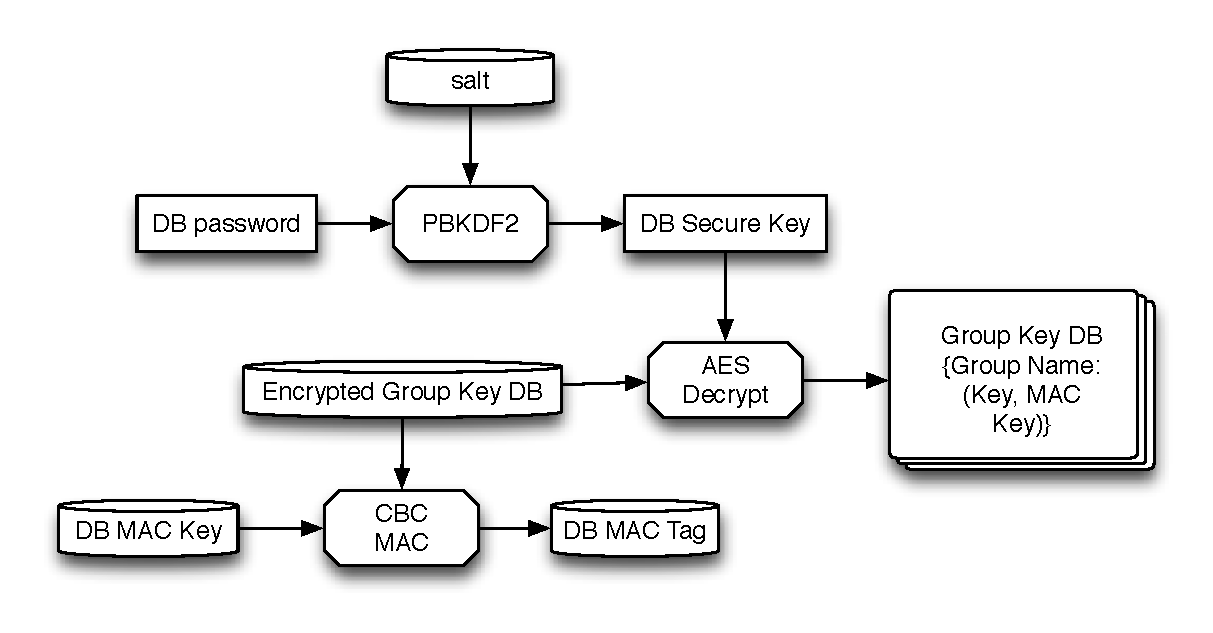
\includegraphics[height=6cm]{fig/db.eps}
\end{figure}

\subsection{How we implement the block cipher for group message and make sure it is safe against CPA attack?}
We implemented nonce-based counter mode (CTR) using AES to encrypt and decrypt group messages using the group keys, which is shown in figure \ref{fig:msg_enc} and \ref{fig:msg_dec}. 
For integrity, we use the MAC with a seperate key to ensure the integrity of the data. We send the MAC tag with the ciphertext together.

By Counter-mode Theorem, since $AES$ is a secure PRP over $(K,X,X)$, CTR has semantic security under $q$ queries of CPA over $(K,X^L,X^{L+1})$ as long as $q^2L \ll |X|$. 
So such mode is proved to be secure.

\begin{figure}[h!]
\centering
\caption{Encryption of group message}
\label{fig:msg_enc}
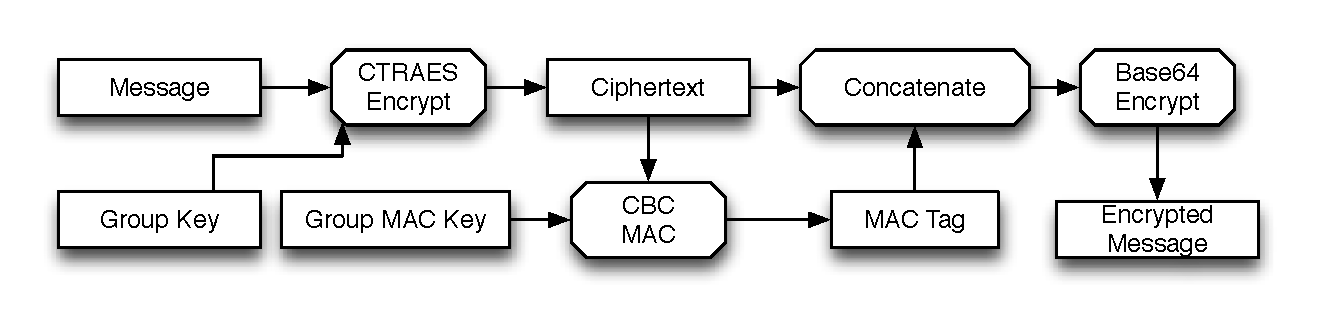
\includegraphics[width=12cm]{fig/msg_enc.eps}
\end{figure}
\begin{figure}[h!]
\centering
\caption{Decryption of group message}
\label{fig:msg_dec}
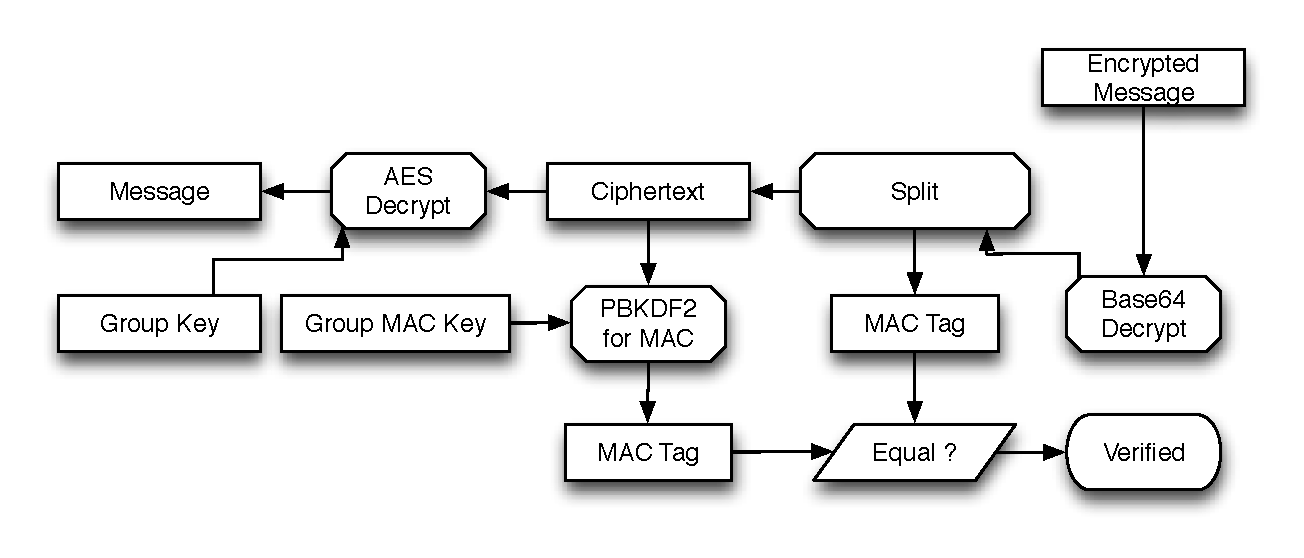
\includegraphics[width=12cm]{fig/msg_dec.eps}
\end{figure}

\subsection{What would happen if the attacker has access to localStorage and other locally stored materials? }
The assumption here is that the attacker has access to all locally stored materials after the user closes the session (browser tab). Namely, the locally stored information includes the encrypted database of  group keys, the salt of the database password, the MAC key, and the MAC tag for the encrypted database password. The attacker can not get significant information about the group keys because the encrypted database key is not stored locally, and he can not recover the encrypted database key from a secure MAC function without exhaustive search. He's not able to understand the encrypted database without knowing the encrypted database key since the nonce-based counter mode is secure under CPA attack. 
\subsection{How we implement the block padding?}

\begin{figure}[h!]
\centering
\caption{Padding a message}
\label{fig:padding}
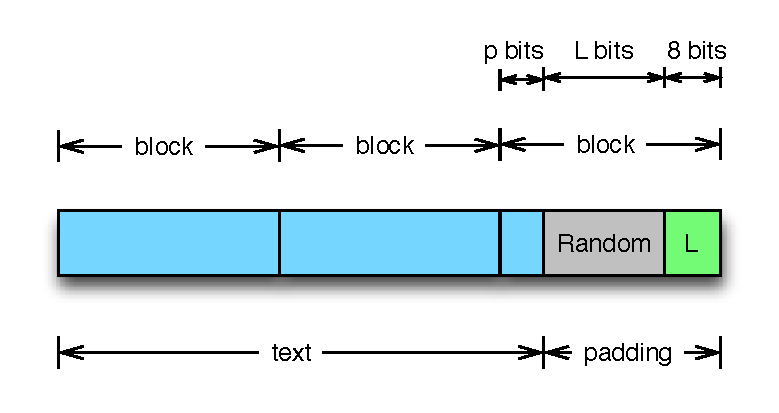
\includegraphics[width=8cm]{fig/padding.eps}
\end{figure}

The figure \ref{fig:padding} shows how we implement the block padding. We suppose the block size is 256 bits and the text in the last block is occupied the first $p$ bits. If $p \le 256 - 8$, we set the last byte of the last block is the length $L = 256 - p - 8$ of the random pad. Then we fill $L$ random bits between the last byte and the end of the text. 
If $p > 256 - 8$, we will append a new block, and set the last byte of the last block is the length $L = 512 - p - 8$, and fill $L$ random bits between the last byte and the end of the text. 

\subsection{How we generate keys?}
The \texttt{Math.random()} function from javascript is not random. So we use the \texttt{crypto} library from Chrome to generate random keys. In \texttt{GenerateKey}, we generate a random key of 512 bits. The first 256 bits are used as the key for the group message encryption, and the last 256 bits are used as the key for MAC of the message encryption. 

\subsection{How could somebody go about circumventing the security of your implementation, if they really wanted to?}
The attacker could use side channel attacks on the computer system to monitor the timing and energy flow on chip of decryption or encryption of the messages to find out the keys. The attackers can also potentially implant viruses or use web browser security holes to steal sessionStorage information from the user or even listen to key strokes on the system level. The attacker can also forge a insecure web browser with their own implementation of web standards and javascript runtime for the user to download and use. Insecurely executed javascript on the browser or injected scripts from untrusted third party would also lead to trivial attacks. Finally, the attacker can deploy generic attack so that he can use the cipher to process huge amount of plaintext until the key is no longer secure (need renew key at this point).

\subsection{What are some of the biggest issues with doing cryptography in the browser? Why might we want to do it anyhow?} 

The biggest issues might be that the designer of the \texttt{crypto} program and the web system using the \texttt{crypto} library on the client has no control on the user behavior and other programs running on the client. A mistakenly implemented web browser might leak session storage; A malicious piece of software can monitor system memory to sniff data loads and store; A website can forge the exact same look and feel to trick the user to use other systems unintentionally; A browser plugin can inject unsecure javascript to the browser, etc.

We might still want to do it anyhow because \texttt{crypo} on the client saves the computational resources on the server side of the system. It also brings the benefit of separating modules from larger systems to maintain less layer of server logic and better isolation of code logic. In addition, when the server end is compromised, the service does not lose important user information if sensitive encrypted keys are stored on the client locally.

\section{Instruction to using the system}

\subsection{Running Program}

We created our own UI imitating the original facebook style. We designed the UI to follow the exact requirement of this assignment. Namely, when user logs in, she has to setup a database password if she hasn't done so. Once the password is setup, she has to enter the password to proceed to view the page on each new browser tab. If the password is wrong, she won't be able to continue and the UI reflects the wrong password. If no key is found in a group, we show a message box to indicate the user to create one. 
We didn't change the workflow of group key creation. So the user, say $A$, could generate a new group key in account setting page. If the other user $B$ want to see the encrypted message sent by $A$, she has to add the same group key of $A$ in $B$'s account setting page.

\subsection{Code}

We didn't change \texttt{menifest.json} except modifying the javascript file name and adding our names to the description.

We didn't make any change to the code below \texttt{GetRandomValues()} and we implemented the required functions (\texttt{Encrypt}, \texttt{Decrypt}, \texttt{GenerateKey}, \texttt{SaveKeys}, \texttt{LoadKeys}) in the assignment. We added several helper functions under \texttt{LoadKeys()}, their main purposes are building UI (\texttt{BuildUIBox}), initiating and querying database password (\texttt{GetDBSecurePassword}), calculate padding (\texttt{Unpadding}, \texttt{Padding}), and implement the nounce-based counter mode (\texttt{CTRAESDecript}, \texttt{CTRAESEncript}). It's easy to see the documentation in the code to learn what they do.

\subsection{Comment}

Because localStorage is not shared over two protocols http and https even under the same domain ``facebook.com''. 
The starter code implements a localStorage that actually stores the data into the shared persistent chrome.storage with caching in the localStorage of the browsing page. But it does not implement the data synchronization between caches of different protocols. Thus, after modifying the group key in the account setting page (https), we cannot immediately get the group key in the group page (http), unless refreshing the tab. So, in our implementaion, we force to redirect user to the https page. 

\end{document}

